\documentclass{beamer}
\setbeamertemplate{caption}[numbered]
\usetheme{Malmoe}
\useoutertheme{infolines} % To have section title in top

\usepackage[backend=bibtex]{biblatex}
\usepackage{listings}
\usepackage{sansmathaccent}
\usepackage{graphicx}
\pdfmapfile{+sansmathaccent.map}
\bibliography{readings}

\def\arraystretch{1.1}%  1 is the default, change whatever you need
\newcommand{\specialcell}[2][c]{%
	\begin{tabular}[#1]{@{}c@{}}#2\end{tabular}}
\newcommand{\code}[1]{\texttt{#1}}

%\AtBeginSection[]
%{
%	\begin{frame}
%		\frametitle{Table of Contents}
%		%\tableofcontents[currentsection,subsectionstyle=show/shaded/hide]
%	\end{frame}
%}

\AtBeginSubsection[]
{
	\begin{frame}
		\frametitle{Table of Contents}
		\tableofcontents[currentsection,currentsubsection]
	\end{frame}
}

\title[Prometheus AI] % (optional, only for long titles)
{Prometheus AI}
\subtitle{Phase 1}
\author[Sean Stappas] % (optional, for multiple authors)
{Sean Stappas
	\\{\small Supervised by: Prof. Joseph Vybihal}}
\date[March 30, 2017] % (optional)
{ECSE-498 Presentation}
\subject{Computer Science}

\begin{document}
	\lstset{language=Java} 
	\beamertemplatenavigationsymbolsempty
	\frame{\titlepage}
	
	\begin{frame}
		\frametitle{Table of Contents}
		\tableofcontents
	\end{frame}
	
	\section{Problem description}
	
	\subsection{Motivation}
	
	\begin{frame}
		\frametitle{Swarm Robotics}
		\framesubtitle{Coordinating multiple robots}
		The aim is to create an intelligent system controlling multiple agents simultaneously working in a swarm. Possible applications include robots in hazardous environments:
		\begin{enumerate}
			\item Outer space (Moon, Mars)
			\item Nuclear disaster aftermath
			\item Oil pipeline inspection
			\item Military zones
		\end{enumerate}
	\end{frame}
	
	\subsection{Prometheus AI Model}
	
	\begin{frame}
		\frametitle{Prometheus AI}
		\framesubtitle{A model of the human brain}
		The Prometheus AI model aims to mimic the basic structure of the human brain with four layers:
		\begin{enumerate}
			\item Neural Network
			\item Knowledge Node Network
			\item Expert System
			\item Meta Reasoner
		\end{enumerate}
	\end{frame}

	\begin{frame}
		\begin{figure}
			\centering
			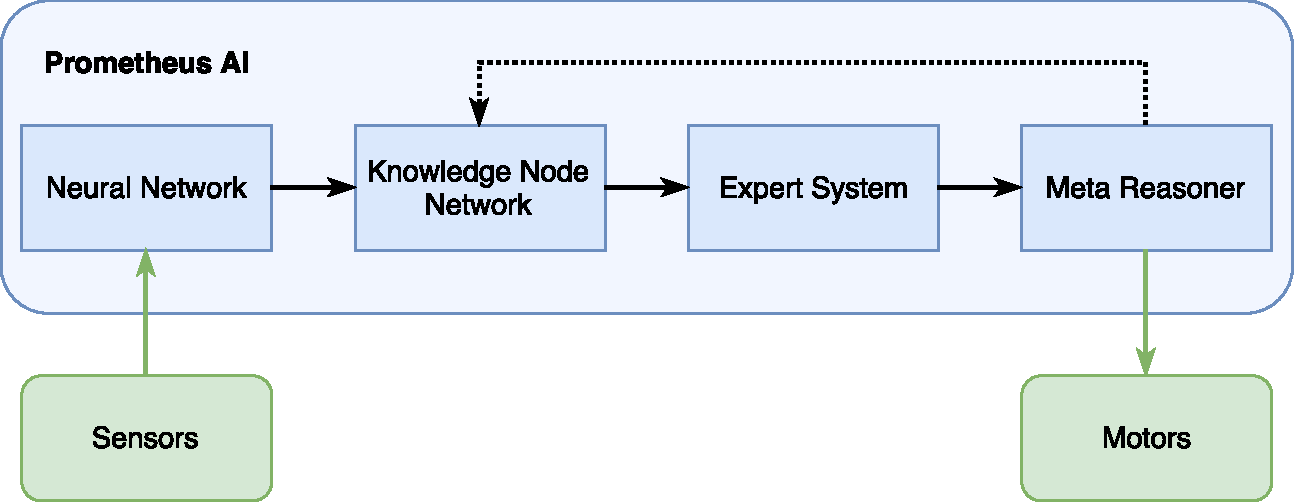
\includegraphics[width=\textwidth]{figures/ai_model.pdf}
			\caption
			{Full AI model.}
			\label{fig:full_model}
		\end{figure}
	\end{frame}

	\begin{frame}
		\frametitle{1. Neural Network}
		The Neural Network (NN) is a \textbf{signal classifier} and the first interface between the sensors and the rest of the system.
		\begin{description}
			\item[input] Signals from the robots' sensors (through an external API).
			\item[output] Tags to be used by the Knowledge Node Network.
			%\item[output] Simple tuples of \code{(label, measurement)}.
		\end{description}
		\begin{figure}
			\centering
			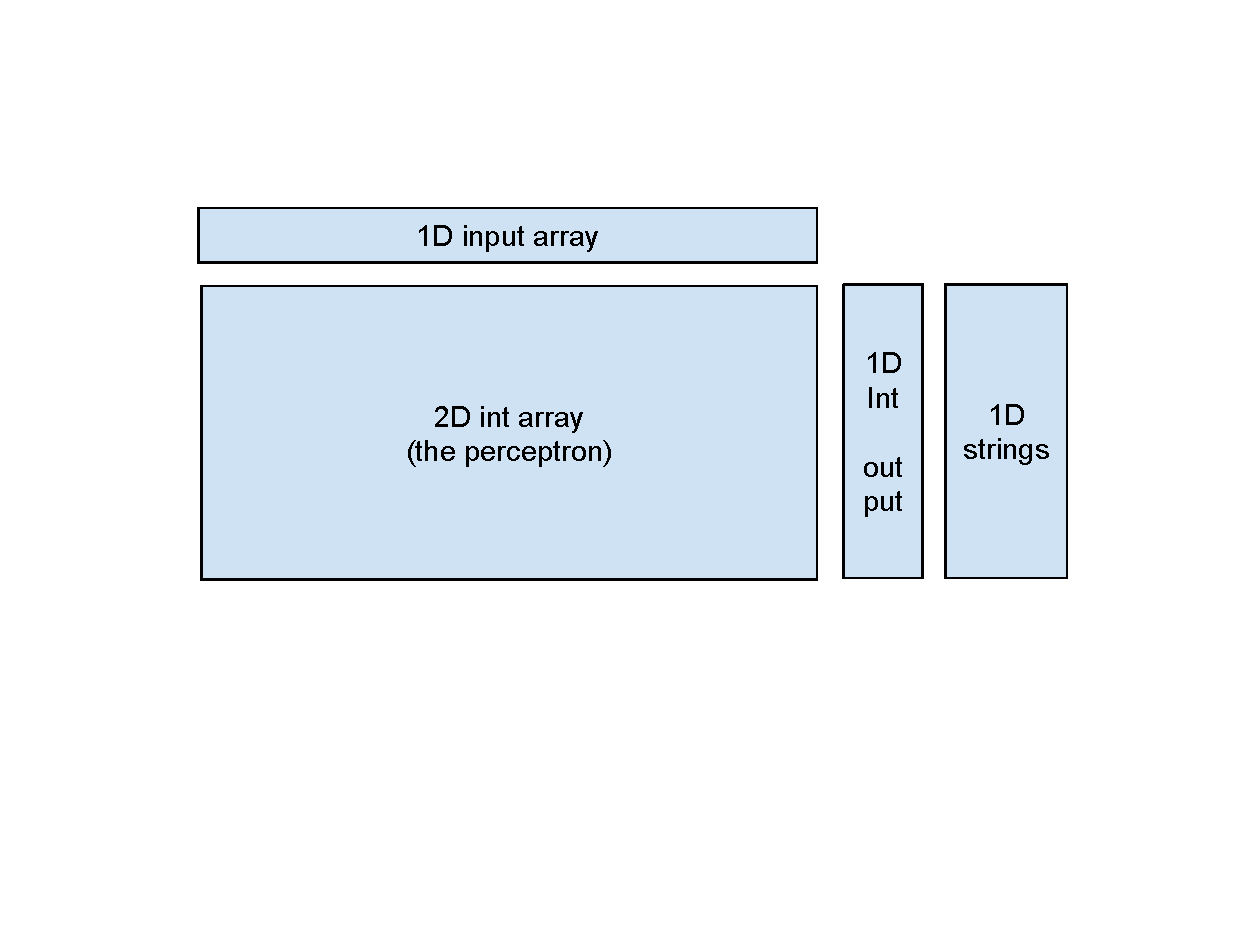
\includegraphics[width=0.6\textwidth]{figures/perceptron.pdf}
			\caption
			{A perceptron \footfullcite{vybihal-model}.}
			\label{fig:perceptron}
		\end{figure}
	\end{frame}

	\begin{frame}
		\frametitle{2. Knowledge Node Network}
		The Knowledge Node Network (KNN) represents \textbf{memory} with the following incomplete list of features \footfullcite{vybihal-knowledge}:
		\begin{itemize}
			\item Aging
			\item Spread of activation
			\item Thresholds
			\item Weighted connections
			\item Learning
			\item Effort
			\item Belief
		\end{itemize}
	
		\begin{description}
			\item[input] 
				Tags from the Neural Network. \linebreak
				Commands from the Meta Reasoner.
			\item[output] Tags (facts, recommendations and rules).
		\end{description}
	
	\end{frame}

	\begin{frame}
		\frametitle{Knowledge Node}
		The Knowledge Node Network is centered around the concept of \textbf{Knowledge Nodes}, a one-to-many structure similar to neurons. The input tag represents information and the output tag represents information related to the input tag.
		\begin{figure}
			\centering
			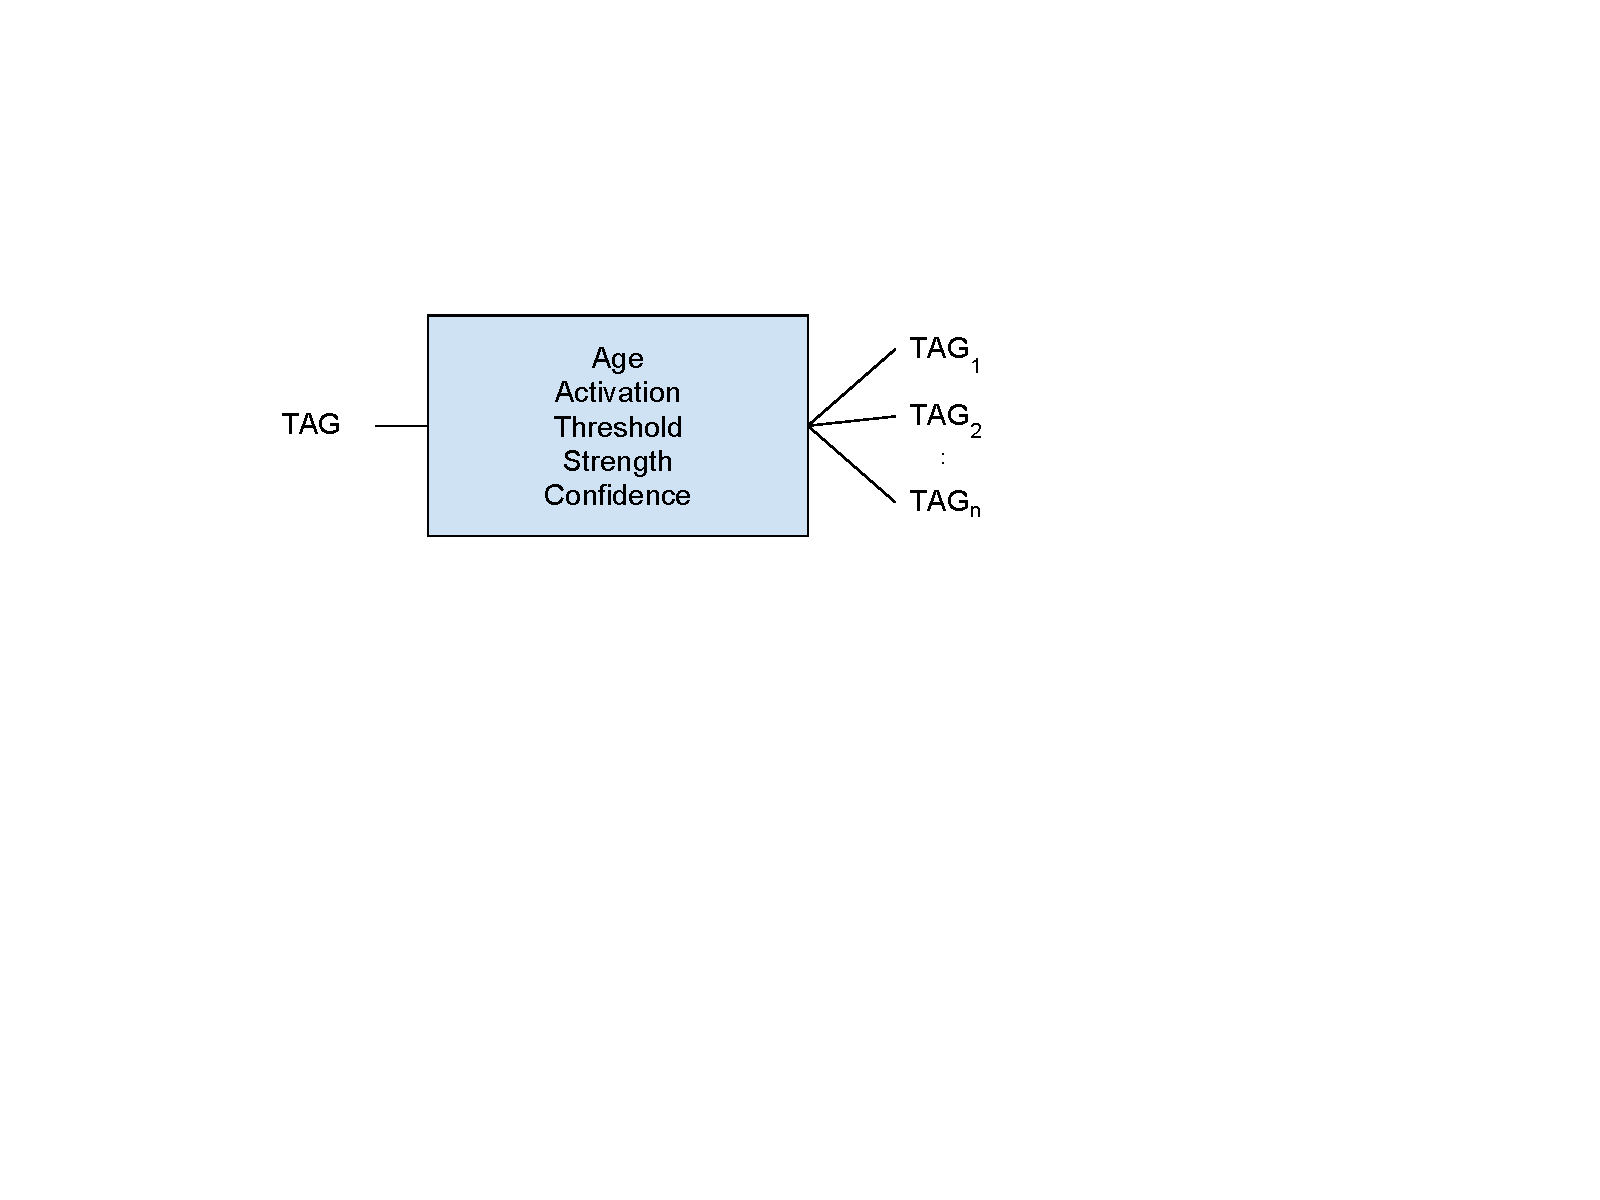
\includegraphics[width=0.8\textwidth]{figures/kn.pdf}
			\caption
			{An abstract view of the Knowledge Node \footfullcite{vybihal-model}.}
			\label{fig:kn}
		\end{figure}
	\end{frame}

	\begin{frame}
		\frametitle{3. Expert System}
		The Expert System (ES) is a \textbf{basic logic reasoner}, unaware of context.
		
		\begin{description}
			\item[input] Tags from the Knowledge Node Network.
			\item[output] Recommendations for actions to take (such as ``turn left'').
		\end{description}
	\end{frame}

	\begin{frame}
		\frametitle{Simple Expert System}
		\begin{table}
			\begin{tabular}{c | c | c | c} 
				\textbf{Facts} & \textbf{Ready Rules} & \textbf{Activated Rules} & \textbf{Fired Tags} \\ \hline
				$(A),(B)$ & \specialcell{$(A)(B) \rightarrow (D)$ \\ $(D)(B) \rightarrow (E)$ \\ $(D)(E) \rightarrow (F)$} & & \\ \hline
				$(A),(B)$ & \specialcell{$(D)(B) \rightarrow (E)$ \\ $(D)(E) \rightarrow (F)$} & $(A)(B) \rightarrow (D)$  & $(D)$ \\ \hline
				$(A),(B),(D)$ & \specialcell{$(D)(E) \rightarrow (F)$} & \specialcell{$(A)(B) \rightarrow (D)$ \\ $(D)(B) \rightarrow (E)$} & $(E)$ \\ \hline
				$\vdots$ & $\vdots$ & $\vdots$ & $\vdots$
			\end{tabular}
			\caption{Example of cascading in a simple expert system \footfullcite{vybihal-expert}}
		\end{table}
	\end{frame}

	\begin{frame}
		\frametitle{4. Meta Reasoner}
		\framesubtitle{High-level thinking}
		The Meta Reasoner (META) receives recommendations from the ES and makes an intelligent decision based on its own \textbf{paranoid} view of the world. The META is aware of context and may reject the KNN's recommendation based on how that action would affect the current reality.
		\linebreak
		
		This layer represents \textbf{high-level thinking} in humans.
		
		\begin{description}
			\item[input] Recommendations from the Expert System.
			\item[output]
				Commands to the robots' motors (through an external API). \linebreak
				Commands to the Knowledge Node Network (think cycle).
			
		\end{description}
	\end{frame}

	\begin{frame}
		\frametitle{Summary}
		\begin{figure}
			\centering
			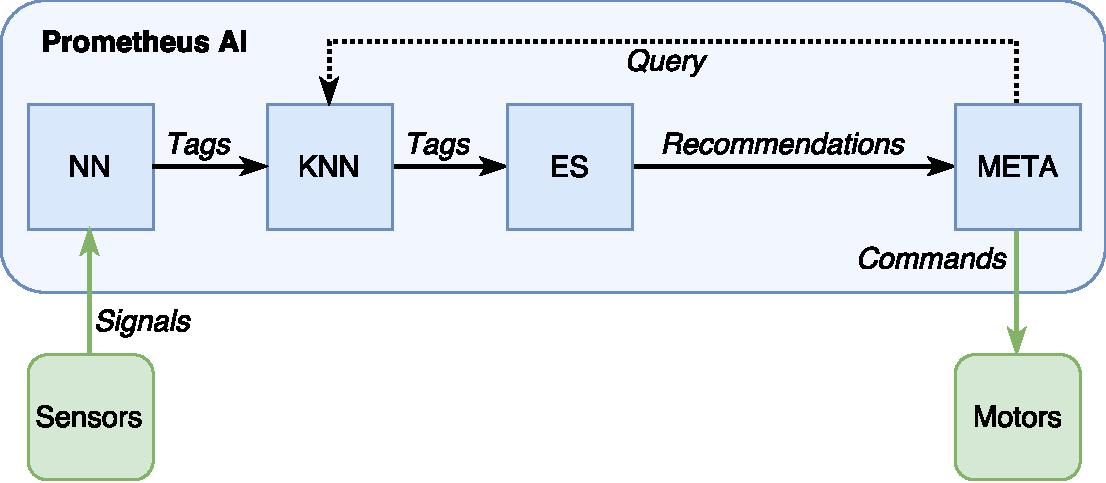
\includegraphics[width=\textwidth]{figures/ai_model_labeled.pdf}
			\caption
			{Summary of the Prometheus AI layers, with emphasis on the input/output of each layer.}
			\label{fig:summary}
		\end{figure}
	\end{frame}

	\subsection{Task}
	
	\begin{frame}
		\frametitle{Assigned Task}
		The task assigned to me was to implement the \textbf{Expert System} and \textbf{Knowledge Node Network} in Java based on some preliminary specifications.
		\linebreak
		
		The other two layers (Neural Network and Meta Reasoner) were to be done in parallel by another student.
	\end{frame}
	
	\section[This semester]{Work done this semester}
	
%	\subsection{Initial Research}
%	
%	\begin{frame}
%		\frametitle{Fundamentals of AI}
%		\framesubtitle{}
%		First I learned about the fundamentals of AI, including Intelligent Agents.
%		\begin{figure}
%			\centering
%			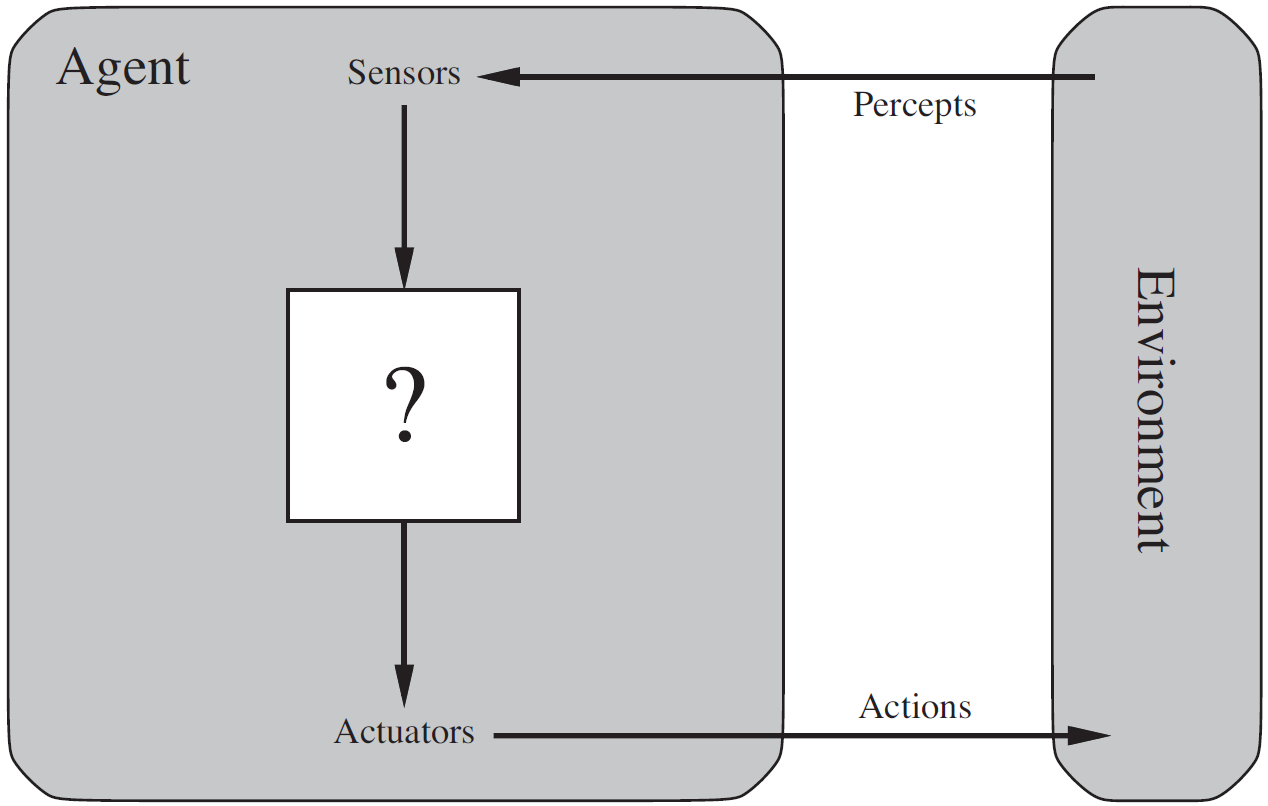
\includegraphics[width=0.6\textwidth]{figures/rational_agents.png}
%			\caption
%			{Rational agents \footfullcite{russell2016artificial}.}
%			\label{fig:rational_agents}
%		\end{figure}
%	\end{frame}
%	
%	\begin{frame}
%		\frametitle{Neural Networks}
%		I read about neural networks, deep learning and stochastic gradient descent.
%		\begin{figure}
%			\centering
%			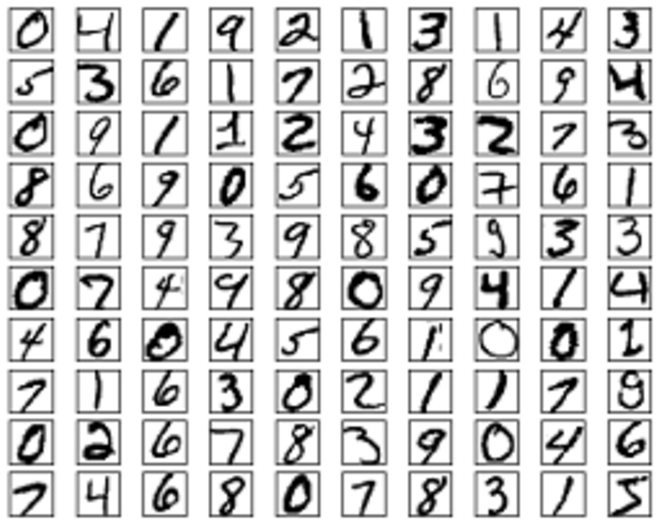
\includegraphics[width=0.4\textwidth]{figures/mnist.png}
%			\caption
%			{MNIST data set. \footfullcite{nielsen2015}.}
%			\label{fig:mnist}
%		\end{figure}
%	\end{frame}
	
	\subsection{Design}
	
	\begin{frame}
		\frametitle{Weekly Meetings}
		Weekly meetings were conducted to assess progress in the project.
		\begin{figure}
			\centering
			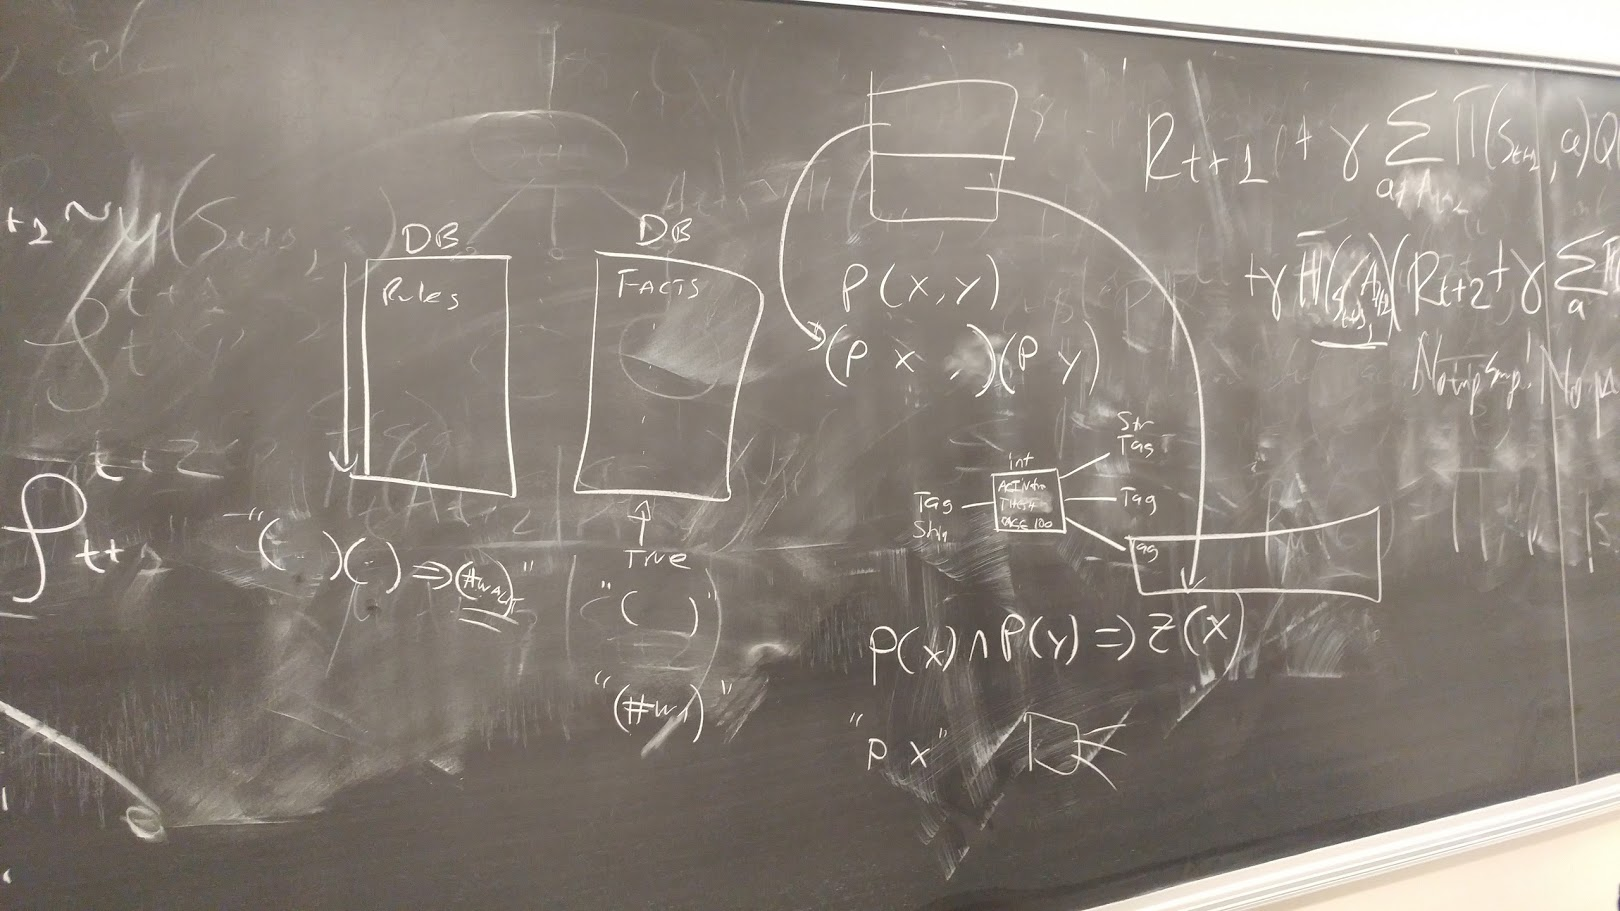
\includegraphics[width=0.9\textwidth]{figures/meeting.jpg}
			\caption
			{One of the weekly discussions on the blackboard.}
			\label{fig:meeting}
		\end{figure}
	\end{frame}
	
	\begin{frame}
		\frametitle{Design Criteria}
		The design of both the Expert System and Knowledge Node Network had many criteria:
		\begin{itemize}
			\item Object-Oriented Design
					\begin{itemize}
						\item Encapsulation
						\item Abstraction
						\item Inheritance
						\item Polymorphism
					\end{itemize}
			\item Efficiency (space \& time)
			\item Documentation (Javadoc) \url{http://cs.mcgill.ca/~sstapp/prometheus/index.html}
		\end{itemize}
	\end{frame}

	\begin{frame}
		\frametitle{Tags}
		The entire system revolves around tags, which can be one of three types:
		\begin{description}[Recommendation]
			\item[Fact] Simple calculus predicate (essentially boolean expression). \emph{e.g.: $(A)$, $(A < 1)$, or $(A = 1)$.}
			\item[Rule] Logical combination of Tags, used by the Expert System. \emph{e.g.: $(A)(B)\rightarrow(C)$.}
			\item[Recommendation] Action to be performed. \emph{e.g.: (\#turn\_left).}
		\end{description}
		To follow object-oriented design, \textbf{Fact}, \textbf{Rule} and \textbf{Recommendation} classes were created, which all subclass an abstract \textbf{Tag} class.
	\end{frame}

	\begin{frame}
		\begin{figure}
			\centering
			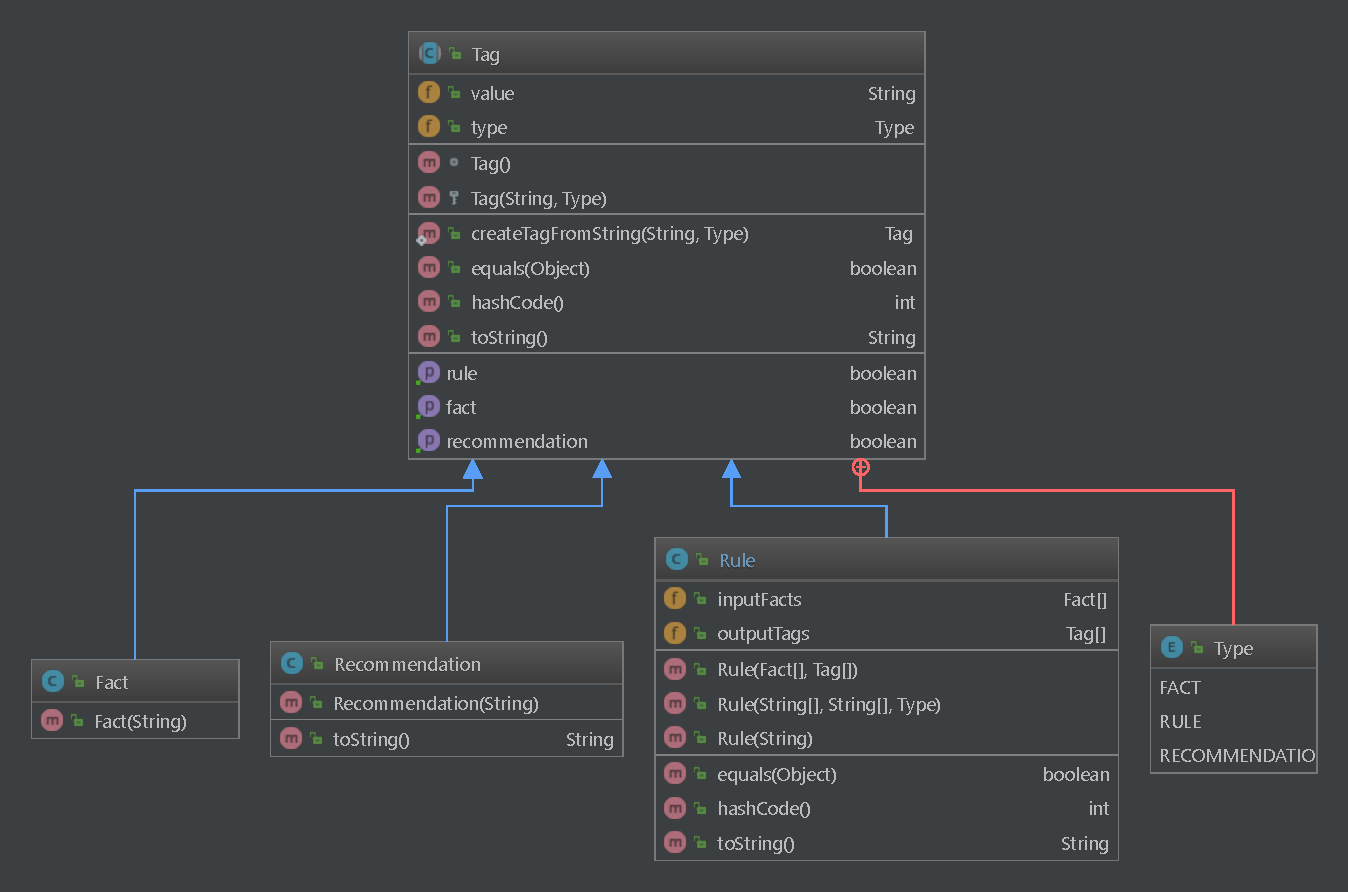
\includegraphics[width=0.9\textwidth]{figures/uml_tags.pdf}
			\caption
			{UML diagram of the \code{tags} package.}
			\label{fig:uml_tags}
		\end{figure}
	\end{frame}
	
	\subsection{Knowledge Node Network}
	
	\begin{frame}
		\frametitle{Terminology}
		We will assume the following terminology for the Knowledge Node Network:
		\begin{description}
			\item[KNN] Knowledge Node Network.
			\item[KN] Knowledge Node.
			\item[active] Describes a Tag that is seen as true by the KNN. If the Tag is the input of a Knowledge Node, it will excite that node (increasing its \code{activation} parameter).
			\item[fired] Describes a Knowledge Node whose \code{activation $\geq$ threshold}.
		\end{description}
	\end{frame}

	\begin{frame}
		\frametitle{Knowledge Node}
		The Knowledge Node has the following important fields:
		\begin{description}
			\item[\code{inputTag}] Represents information and is used as an index.
			\item[\code{outputTags}] Array of output Tags.
			\item[\code{activation}] Integer starting at 0, incrementing when KN is excited. Could also be implemented with sigmoid.
			\item[\code{threshold}] Threshold such that \code{activation $\geq$ threshold} causes firing of the KN.
			\item[\code{strength}] Biases the activation of a KN, causing early firing. Related to learning. Simple implementation: if \code{activation * strength $\geq$ threshold} then fire the KN.
			\item[\code{confidence}] Belief that \code{inputTag} is true (0 to 100\%). Could be associated with each Tag.
			\item[\code{age}] Age of the KN. If greater than some threshold, the KN is discarded.
		\end{description}
	\end{frame}
	
	\begin{frame}
		\frametitle{Data Structures}
		The Knowledge Node Network has the following important data structures:
		\begin{description}[\code{activeTagsMETA}]
			\item[\code{mapKN}] Map of input Tags to associated Knowledge Nodes
			\item[\code{activeTags}] Set of active Tags, corresponding to input Tags of fired Knowledge Nodes
			%\item[\code{activeTuplesNN}] Set of active tuples coming from the Neural Network layer.
			%\item[\code{activeTagsMETA}] Set of active Tags coming from the META layer. These are commands coming from higher up.
		\end{description}
	\end{frame}

	\begin{frame}
		\frametitle{\code{think()}}
		Starts the activation process. The KNN has three main ways of thinking:
		\begin{itemize}
			\item \code{thinkForwards()}
			\item \code{thinkBackwards()}
			\item \code{thinkLambda()}
		\end{itemize}
		The KNN picks the correct way of thinking based on a command from META.
		\begin{description}
			\item[parameters:] A \textbf{number of cycles} can be passed as a parameter to an overloaded version of \code{think()}. This number of cycles represents the amount of \emph{effort} being put into thinking, running until energy-based quiescence \footfullcite{vybihal-knowledge} occurs. Otherwise, \code{think()} takes no parameters and runs to natural quiescence.
			\item[returns:] The Set of Tags activated as a result of thinking.
		\end{description}
	\end{frame}

	\begin{frame}
		\frametitle{\code{thinkForwards()}}
		Forwards thinking is the simplest method. It is based on simple forward activation, similar to the Expert System. If the input Tag of a Knowledge Node is known to be true, then the output Tags become \emph{active} and all the Knowledge Nodes associated with those Tags are \emph{fired}.
		\begin{figure}
			\centering
			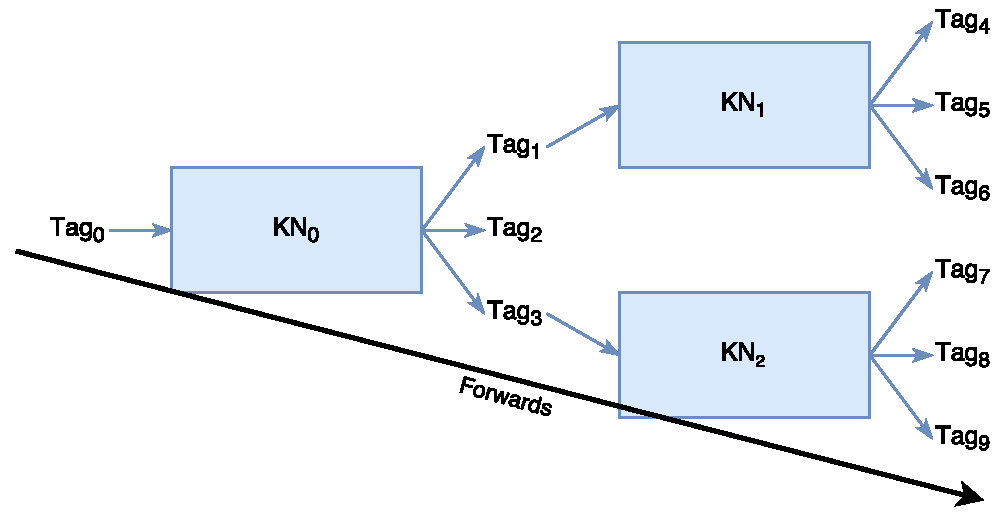
\includegraphics[width=0.65\textwidth]{figures/forwards_thinking.pdf}
			\caption
			{Thinking forwards.}
			\label{fig:forwards_thinking}
		\end{figure}
	\end{frame}

	\begin{frame}
		\frametitle{\code{thinkBackwards()}}
		Backwards thinking looks at the output Tags of Knowledge Nodes and propagates activation backwards. This type of thinking occurs constantly in the background in humans \footfullcite{vybihal-knowledge}.
		\begin{figure}
			\centering
			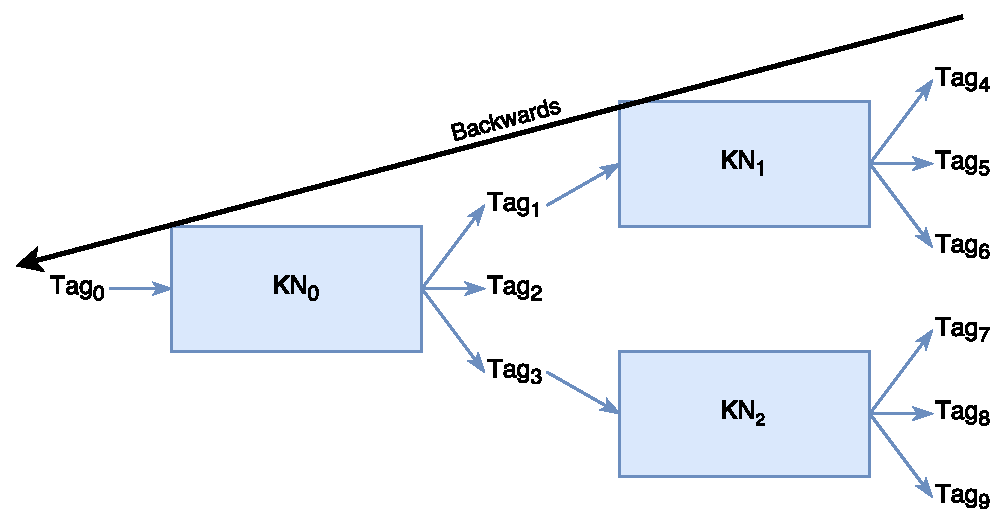
\includegraphics[width=0.65\textwidth]{figures/backwards_thinking.pdf}
			\caption
			{Thinking backwards.}
			\label{fig:backwards_thinking}
		\end{figure}
	\end{frame}
	
	\begin{frame}
		\frametitle{\code{thinkLambda()}}
		The most complex way of thinking, representing a combination of \code{thinkBackwards()} and \code{thinkForwards()}. Commonly used in humans when using analogical reasoning to solve a problem \footfullcite{vybihal-lambda}.
		\begin{figure}
			\centering
			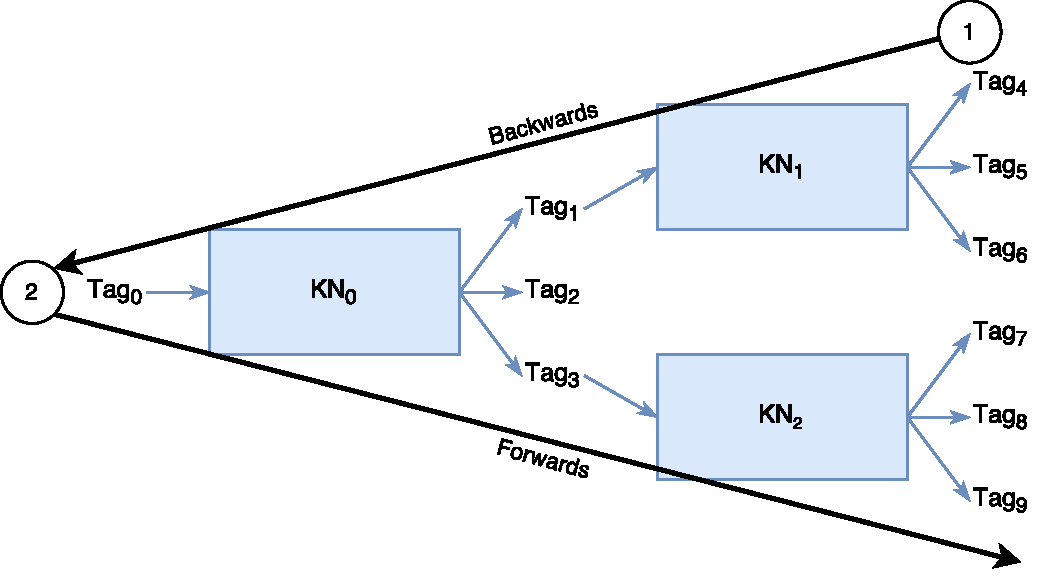
\includegraphics[width=0.65\textwidth]{figures/lambda_thinking.pdf}
			\caption
			{Lambda ($\Lambda$) thinking.}
			\label{fig:lambda_thinking}
		\end{figure}
	\end{frame}
	
	\begin{frame}
		\begin{figure}
			\centering
			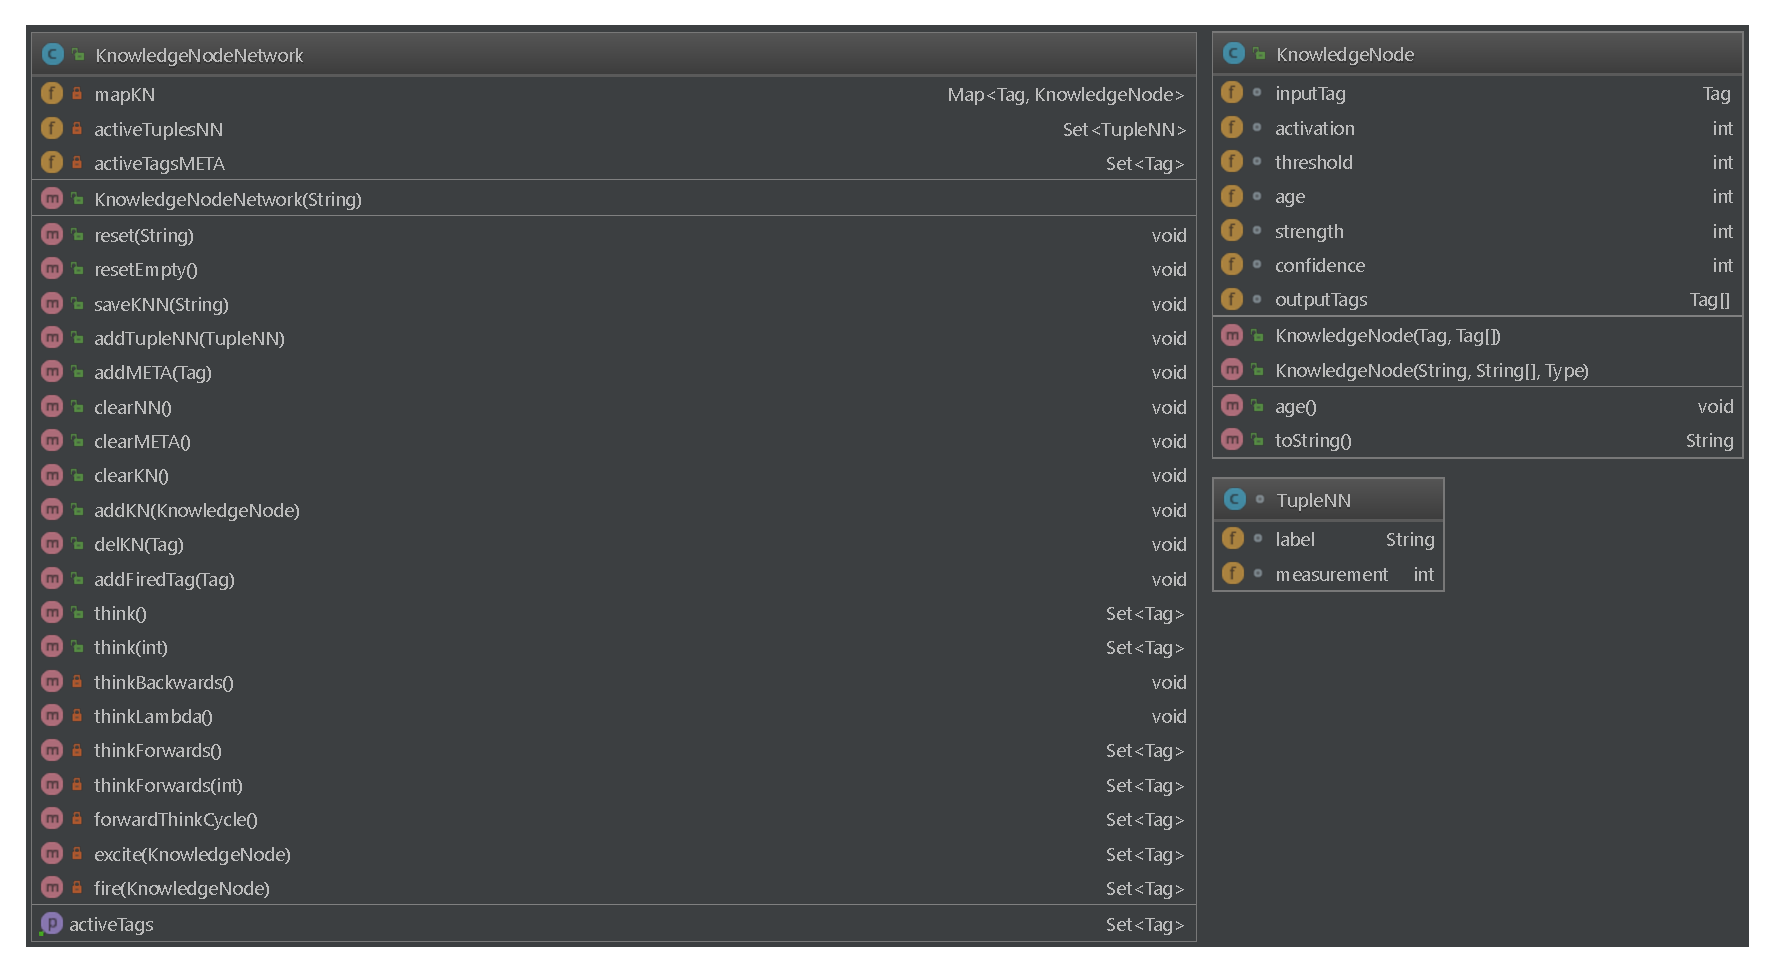
\includegraphics[width=\textwidth]{figures/uml_knn.pdf}
			\caption
			{UML diagram of the \code{knn} package.}
			\label{fig:uml_knn}
		\end{figure}
	\end{frame}
	
	\subsection{Expert System}
	
	\begin{frame}
		\frametitle{Terminology}
		We will assume the following terminology for the Knowledge Node Network:
		\begin{description}
			\item[ES] Expert System.
			\item[active Tag] A Fact or Recommendation that is seen as true by the ES. If all input Tags of a Rule are active, that Rule will become active.
			\item[active Rule] A Rule whose input Tags are active, making its output Tags active.
			\item[ready Rule] A Rule that has not yet become active.
			\item[to activate] To make a Tag or Rule active.
		\end{description}
	\end{frame}
	
	\begin{frame}
		\frametitle{Rule}
		The Expert System is based around cascaded activation of Rules, a many-to-many structure. A Rule has the following important fields:
		\begin{description}
			\item[\code{inputTags}] Array of input Tags representing the conditions of the Rule.
			\item[\code{outputTags}] Array of output Tags, which become active when \textbf{all} condition Tags are active (logical AND).
		\end{description}
	
		\begin{equation}
			(Tag_{in_1}) \cdots (Tag_{in_m}) \rightarrow (Tag_{out_1}) \cdots (Tag_{out_n})
		\end{equation}
	\end{frame}

	\begin{frame}
		\frametitle{Data Structures}
		The Expert System has the following important data structures:
		\begin{description}[\code{recommendations}]
			\item[\code{readyRules}] Set of Rules that have not been activated yet.
			\item[\code{activeRules}] Set of active Rules.
			\item[\code{facts}] Set of active Facts.
			\item[\code{recommendations}] Set of active recommendations.
		\end{description}
	\end{frame}

	\begin{frame}
		\frametitle{\code{think()}}
		Starts the activation process, similarly to the KNN, with the following important differences:
		\begin{itemize}
			\item A rule is either active or not; there is no activation threshold.
			\item Rules are many-to-many; Knowledge Nodes are one-to-many.
			\item The propagation is only forwards (no backwards or lambda).
		\end{itemize}
	
		\begin{description}
			\item[parameters:] A number of cycles can be passed, similarly to the KNN. Otherwise, think() takes no parameters and runs to natural quiescence.
			\item[returns:] The Set of \textbf{Recommendations} activated as a result of thinking. These Recommendations are passed on to the META layer.
		\end{description}
		
	\end{frame}

	\begin{frame}
		\begin{figure}
			\centering
			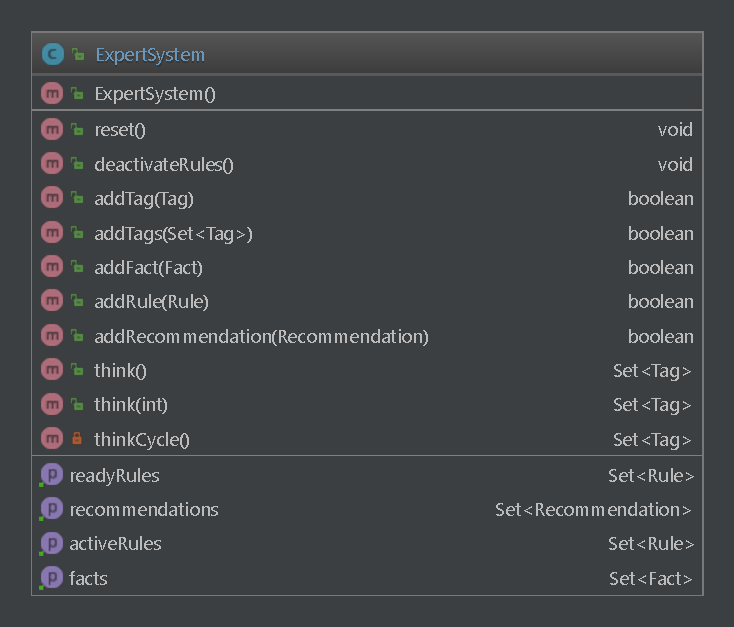
\includegraphics[width=0.7\textwidth]{figures/uml_es.pdf}
			\caption
			{UML diagram of the \code{es} package.}
			\label{fig:uml_es}
		\end{figure}
	\end{frame}

	\subsection{Tests}
	
	\begin{frame}
		\frametitle{Tests}
		Unit tests were created with the TestNG framework
		\begin{description}[\code{TestIntegration}]
			\item[\code{TestES}] Unit tests of all the Expert System methods.
			\item[\code{TestKNN}] Unit tests of the Knowledge Node Network methods.
			\item[\code{TestIntegration}] High-level tests of the ES and KNN (Demo).
			\begin{itemize}
				\item \code{testKNN()}
				\item \code{testES()}
				\item \code{testESandKNN()}
			\end{itemize}
		\end{description}
	\end{frame}

	\begin{frame}
		\frametitle{\code{testES()}}
		\begin{table}
			\small
			\begin{tabular}{c | c | c | c} 
				\textbf{Ready Rules} & \textbf{Active Rules} & \specialcell{\textbf{Active} \\ \textbf{Facts}} & \specialcell{\textbf{Active} \\ \textbf{Recommendations}}  \\ \hline
				\specialcell{$(A)(B)\rightarrow(D)$ \\ $(D)(B)\rightarrow(E)$ \\ $(D)(E)\rightarrow(F)$\\ $(G)(A)\rightarrow(H)$ \\ $(\#X)(\#Y)\rightarrow(\#Z)$} &  & $(A),(B)$ & $(\#X),(\#Y)$ \\ \hline
				$\vdots$ & $\vdots$ & $\vdots$ & $\vdots$ \\ \hline
				$(G)(A)\rightarrow(H)$ & \specialcell{$(A)(B)\rightarrow(D)$ \\ $(D)(B)\rightarrow(E)$ \\ $(D)(E)\rightarrow(F)$ \\ $(\#X)(\#Y)\rightarrow(\#Z)$} & \specialcell{$(A),(B),$ \\ $(D),(E)$ \\ $(F)$} & $(\#X),(\#Y),(\#Z)$		
			\end{tabular}
			\caption{Test setup for \code{testES()}.}
		\end{table}
	\end{frame}

	\begin{frame}
		\frametitle{\code{testKNN()}}
		\begin{figure}
			\centering
			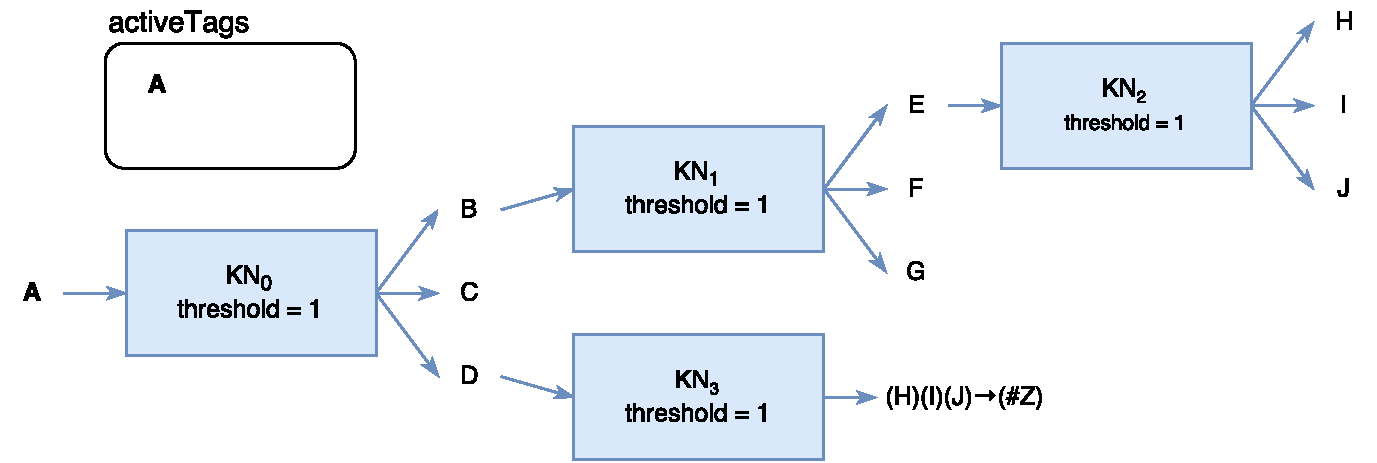
\includegraphics[width=\textwidth]{figures/testKNN.pdf}
			\caption
			{Test setup for \code{testKNN()}.}
			\label{fig:testKNN}
		\end{figure}
	\end{frame}

	\begin{frame}
		\frametitle{\code{testKNNandES()}}
		Same setup as \code{testKNN()}, but the activated Tags are passed on to an Expert System.
		\begin{table}
			\small
			\begin{tabular}{c | c | c | c} 
				\textbf{Ready Rules} & \textbf{Active Rules} & \specialcell{\textbf{Active} \\ \textbf{Facts}} & \specialcell{\textbf{Active} \\ \textbf{Recommendations}}  \\ \hline
				$(H)(I)(J)\rightarrow(\#Z)$
				& 
				& \specialcell{$(B),(C),(D)$ \\ $(E),(F),(G)$ \\ $(H),(I),(J)$}
				& \\ \hline
				
				& $(H)(I)(J)\rightarrow(\#Z)$
				& \specialcell{$(B),(C),(D)$ \\ $(E),(F),(G)$ \\ $(H),(I),(J)$}
				& $(\#Z)$
				
			\end{tabular}
			\caption{Test setup for \code{testKNNandES()}.}
		\end{table}
	\end{frame}

	\begin{frame}
		\begin{figure}
			\centering
			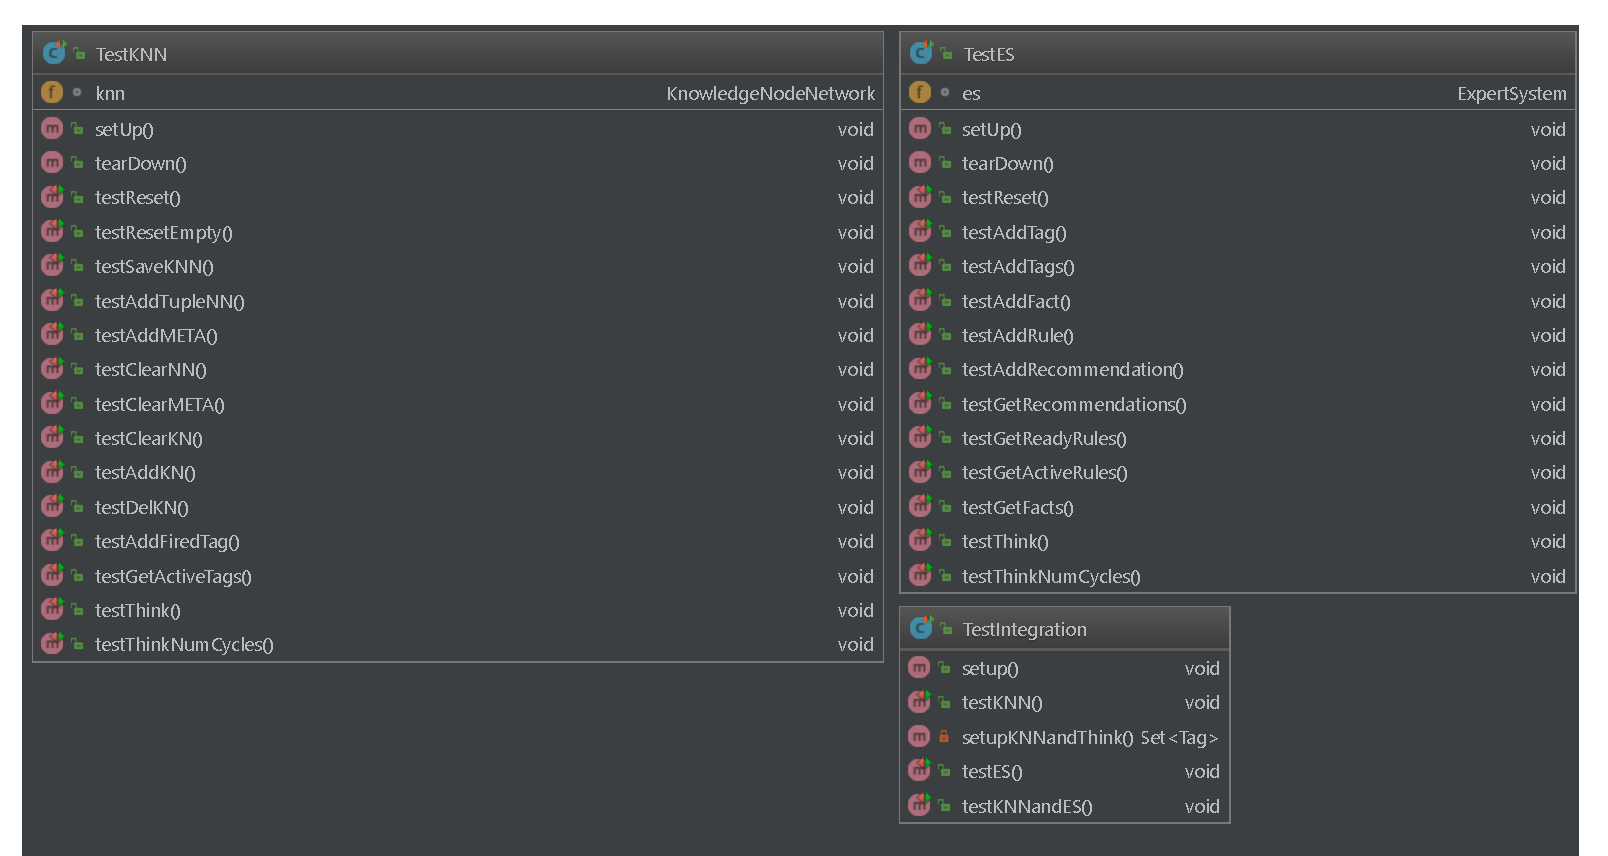
\includegraphics[width=\textwidth]{figures/uml_test.pdf}
			\caption
			{UML diagram of the \code{test} package.}
			\label{fig:uml_test}
		\end{figure}
	\end{frame}
	
	\section[Next semester]{Work plan for next semester}
	
	\subsection{Finalization}
	
	\begin{frame}
		\frametitle{Knowledge Node Network Finalization}
		Some more complex features of the KNN are still to be implemented:
		\begin{itemize}
			\item Lambda thinking
			\item Confidence and strength
			\item Sigmoid activation
			\item Timestamp aging
			\item Interface with Neural Network
		\end{itemize}
	\end{frame}
	
	\begin{frame}
		\frametitle{Expert System Finalization}
		Some features of the Expert System are still to be implemented:
		\begin{itemize}
			\item Fact token matching (=\quad \textless \quad \textgreater)
		\end{itemize}
	\end{frame}

	\subsection{Integration}
	
	\begin{frame}
		\frametitle{Integration}
		The ES and KNN layers will have to be merged with the NN and META, which will probably lead to some conflicts. Time will be required to ensure proper functionality.
	\end{frame}

	\subsection{Testing}
	
	\begin{frame}
		\frametitle{Simulation}
		The Java simulation library Simbad will be used to test the entire system on virtual robots.
		\begin{figure}
			\centering
			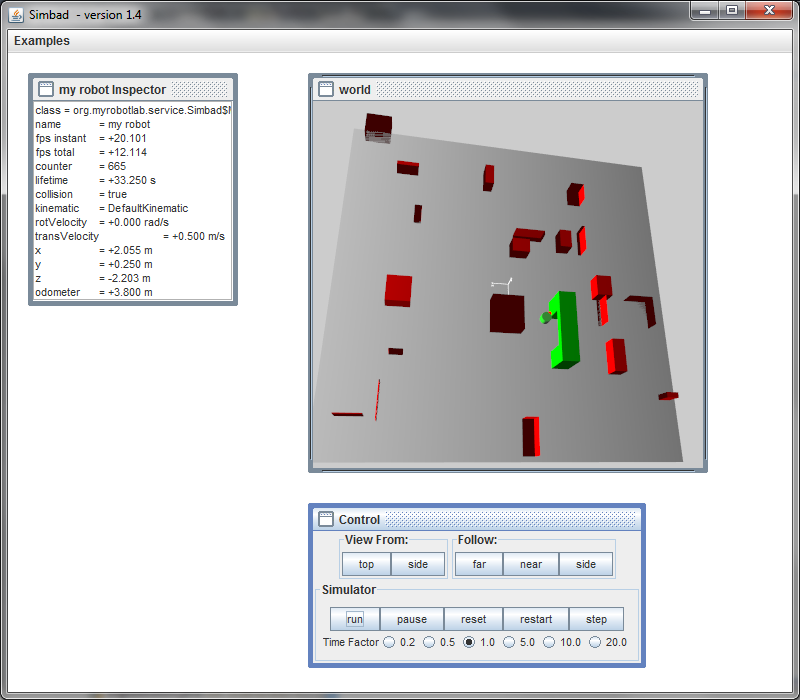
\includegraphics[width=0.5\textwidth]{figures/simbad.png}
			\caption
			{Simbad Java simulator. \footfullcite{simbad}}
			\label{fig:simbad}
		\end{figure}
	\end{frame}

	\begin{frame}
		\frametitle{Physical Testing}
		Prof. Vybihal's lab has multiple simple robots with ultrasonic sensors that can be tested on.
		\begin{figure}
			\centering
			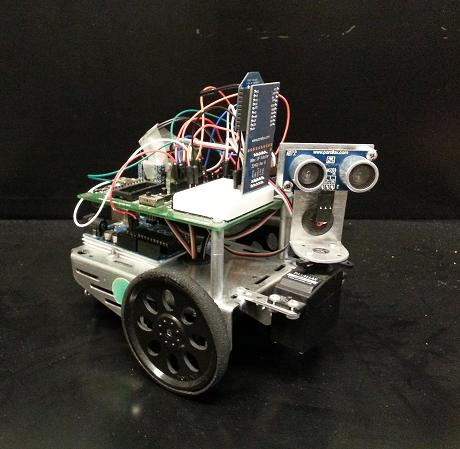
\includegraphics[width=0.5\textwidth]{figures/robot.jpg}
			\caption
			{Robot in the lab.}
			\label{fig:robot}
		\end{figure}
	\end{frame}
	
	\section{References}
	\begin{frame}[t,allowframebreaks]
		\frametitle{References}
		\printbibliography
	\end{frame}
	
\end{document}
